% !TeX root = ../BA_main_englisch.tex
% !TeX spellcheck = en_GB
In this section we examine the higher-dimensional case of $N=5$.
As the data set with $\rho_0 = \ket{+} \bra{+}$, the eigenstate of the Drive Hamiltonian, performed best in the previous section, we focus our attention on this case.
We compare the efficiency of a fully connected ANN (FCANN) to a unidirectional and bidirectional LSTM to analyse the effect of different architectures on the predictive power in our setting.
Both LSTM networks have the same architecture, bar the bi-directionality (see Figure \ref{lstm_network}).
This hyperparameter distinguished the two cases of whether or not the complete drive sequence is known in advance.
Before entering the LSTM cell, each embedded $\ket{\psi_D}$ passes through a two layer FCANN to increase the input dimensionality.
After passing the LSTM a single layer FCANN is applied to the output to produce the embedding size to recover $\ket{\psi_T}$.
The third network uses three fully connected hidden layers, the size of which is selected to approximately match the amount of trainable parameters of the bidirectional LSTM.

The test data efficiency as well as the amount of trainable parameters are presented in Table \ref{n5efftable}.

\begin{figure}
	\centering
	\includegraphics[width=0.7\textwidth]{img/lstm_network}
	\caption{Architecture of the LSTM networks. The green blocks represent the unidirectional case. For the bidirectional case, a second LSTM block (orange) is included with separate trainable parameters. The blocks labeled `FC' represent fully-connected layers.}
	\label{lstm_network}
\end{figure}

\begin{table}[h]
	\centering
	\begin{tabular}{ c | c | c | c | c}
		Network Architecture & $\eta_{test} \ [\%]$ & $\mathrm{MSE}_{test}$ & $W_{test}$ & \# Parameters \\
		\hline
		FCANN        & 19.3 & 0.1083 & 0.53 & 8,086,020 \\
		Bidir. LSTM  & 33.1 & 0.0948 & 0.91 & 7,700,222 \\
		Unidir. LSTM & 19.5 & 0.1707 & 0.52 & 3,206,990\\
	\end{tabular}
	\caption{Efficiencies $\eta$ on the test data for model architectures with given number of trainable parameters for $N=5, \Delta \mathrm{T} = 5$.}
	\label{n5efftable}
\end{table}

The efficiency of the best model for $N=5, \Delta \mathrm{T} = 5$ is drastically lower than that for $N=2$.
Crucially, the models are unable to extract the test set average of the lower bound calculated by local optimisation $W_{lo} = 1.4$.

Contrary to the case of $N=2$, the evolution of the system state becomes relevant over multiple time steps.
As the work per time step is determined by $\mathrm{dW} = -\Tr{\rho_S \ dH} = \Tr{\rho_S (H_{ST}^i - H_{ST}^{i+1})}$, where $H_{ST} = \bra{\psi_D}\bra{\psi_T} \mathds{1}_D \otimes H_I \ket{\psi_D} \ket{\psi_T}$ is the partial system Hamilto-nian acting only between System and Transducer, finding the optimal solution is a compromise of choosing $dH$ so as to maximise the expectation value while controlling the unitary evolution of $\rho_S$ such that $\Tr{\sigma_z \rho_S}$ is small.
We plot the optimal and predicted trajectory of a random data point in the test in Figure \ref{bloch_10553} set to illustrate this compromise.
In \ref{bloch_worst} we plot the trajectories for the worst-performing sample in the test set.
In this case, the prediction for $\ket{\psi_T}$ deviates only slightly from the optimum for $i \in [2, N]$ but deviates significantly for $i=1$.
This illustrates the problem of using the MSE as a cost function for training - to the network, this is a good prediction as most Transducer qubits are near their optimal setting.
The deviation in the first qubit causes a completely different evolution on the system, especially as $\Delta \mathrm{T} = 5$ is large.
This leads to a negative work output when following the predicted protocol.


\begin{figure}
	\centering
	\begin{subfigure}{0.85\textwidth}
		\centering
		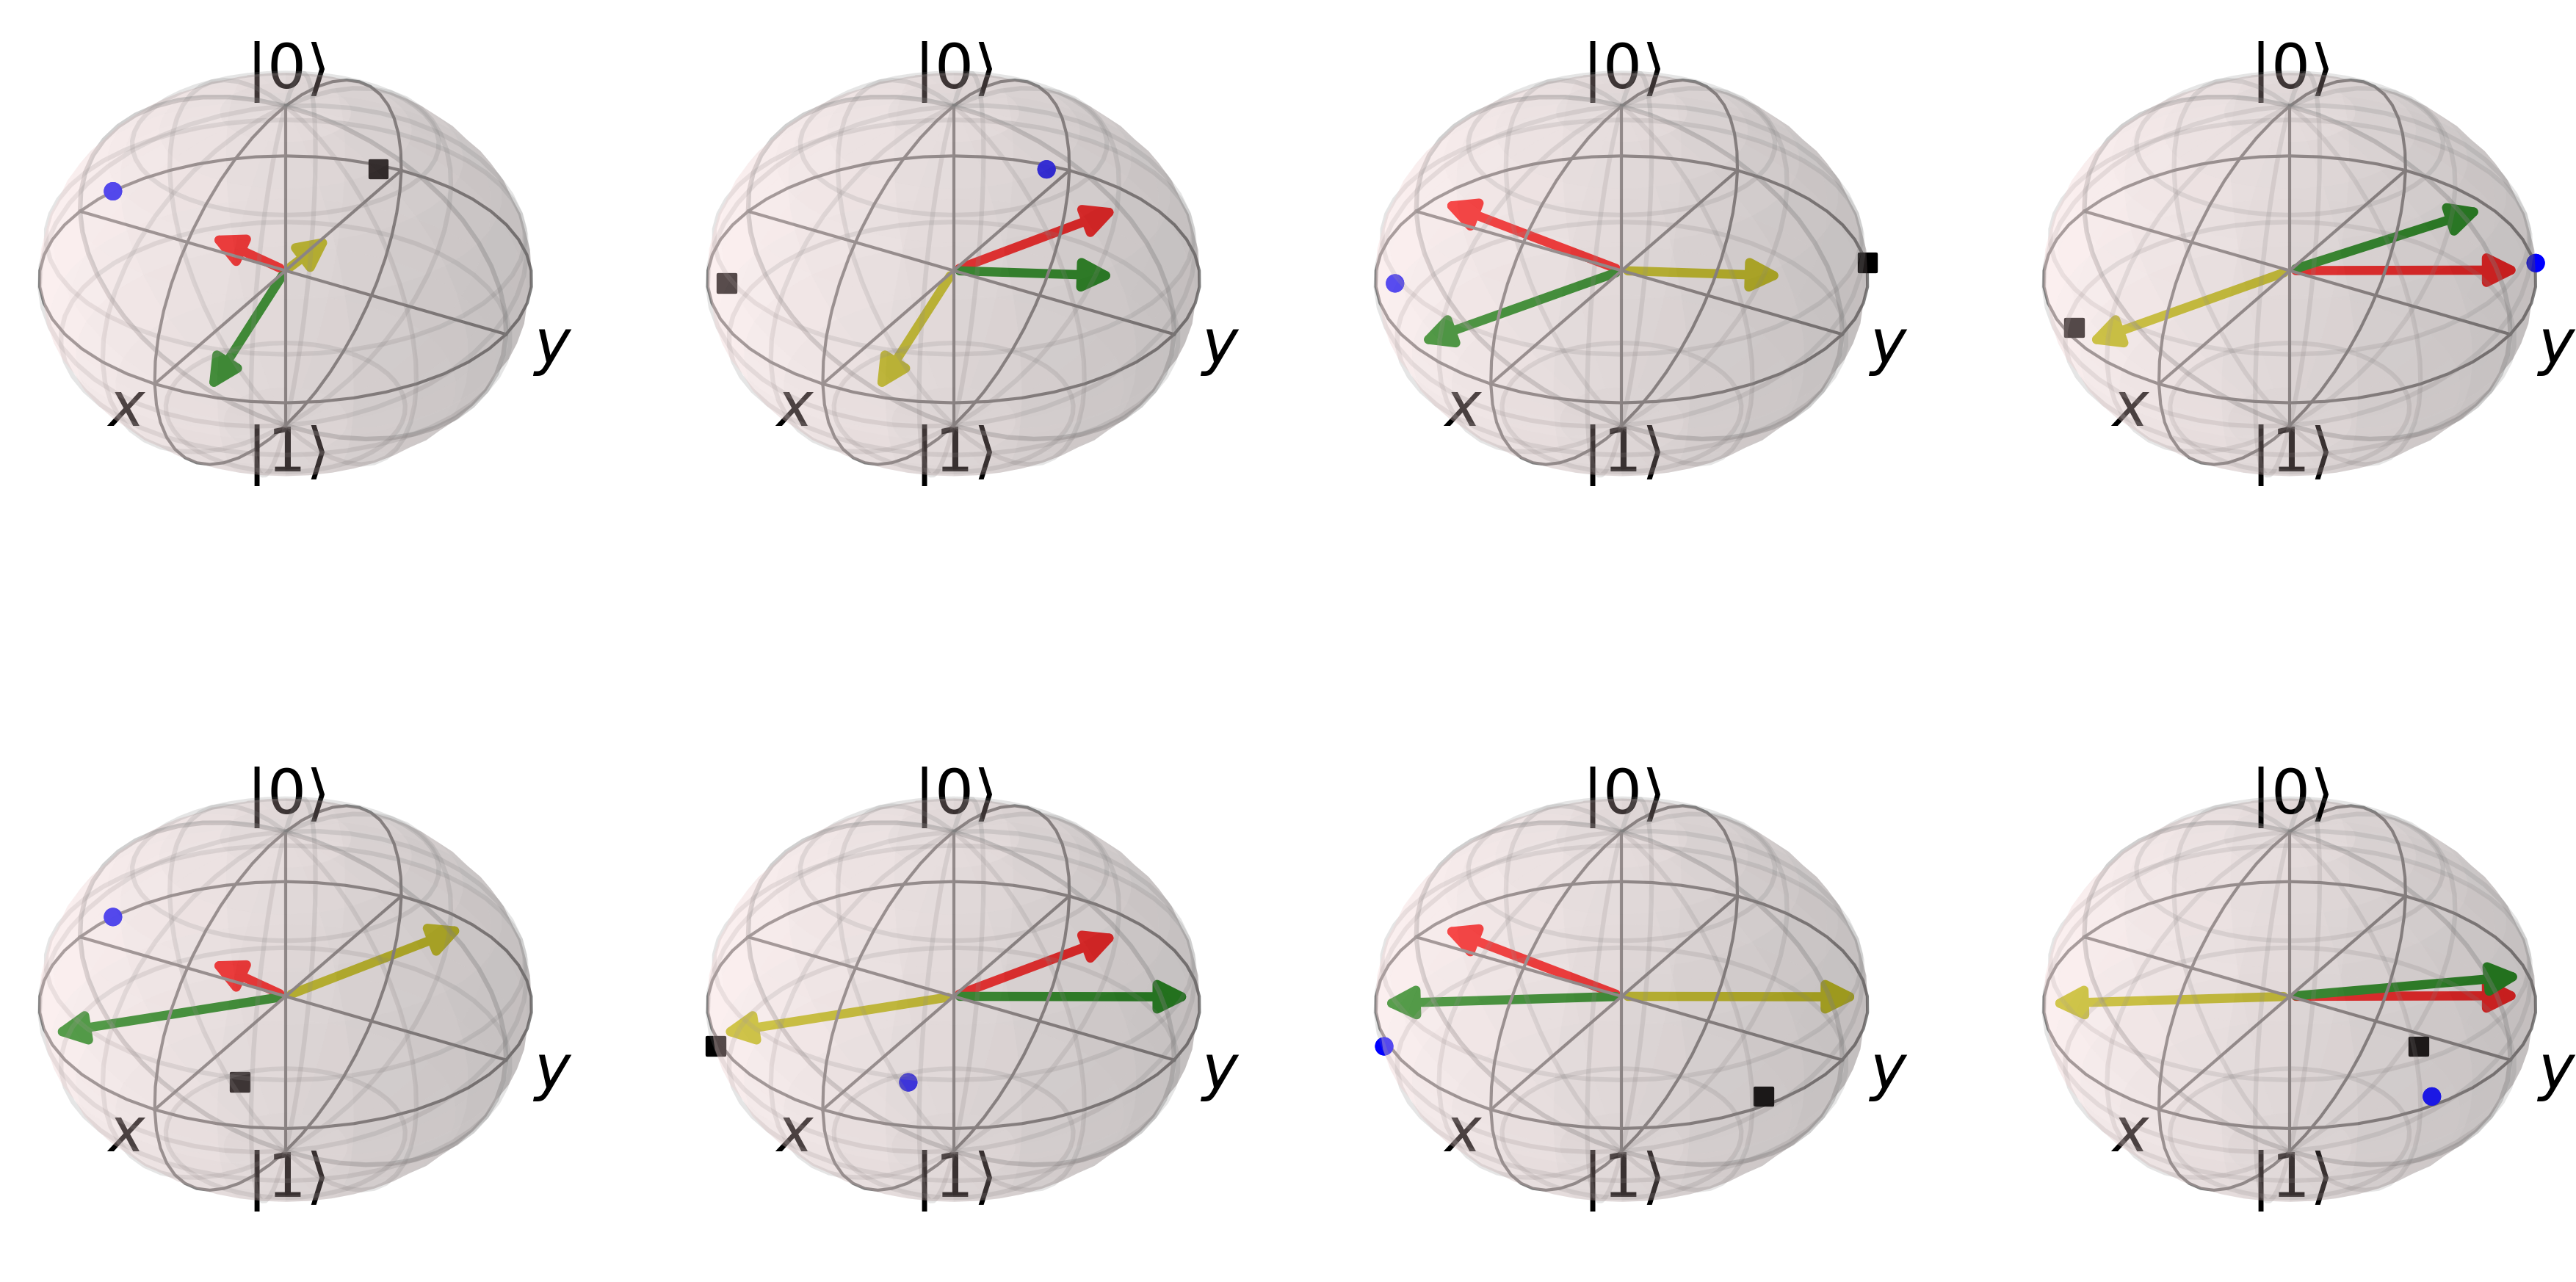
\includegraphics[width=\textwidth]{img/bloch_10553_crop}
		\caption{$W_{opt} = 3.03, W_{pred} = 1.11$}
		\label{bloch_10553}
	\end{subfigure}
	\begin{subfigure}{0.85\textwidth}
		\centering
		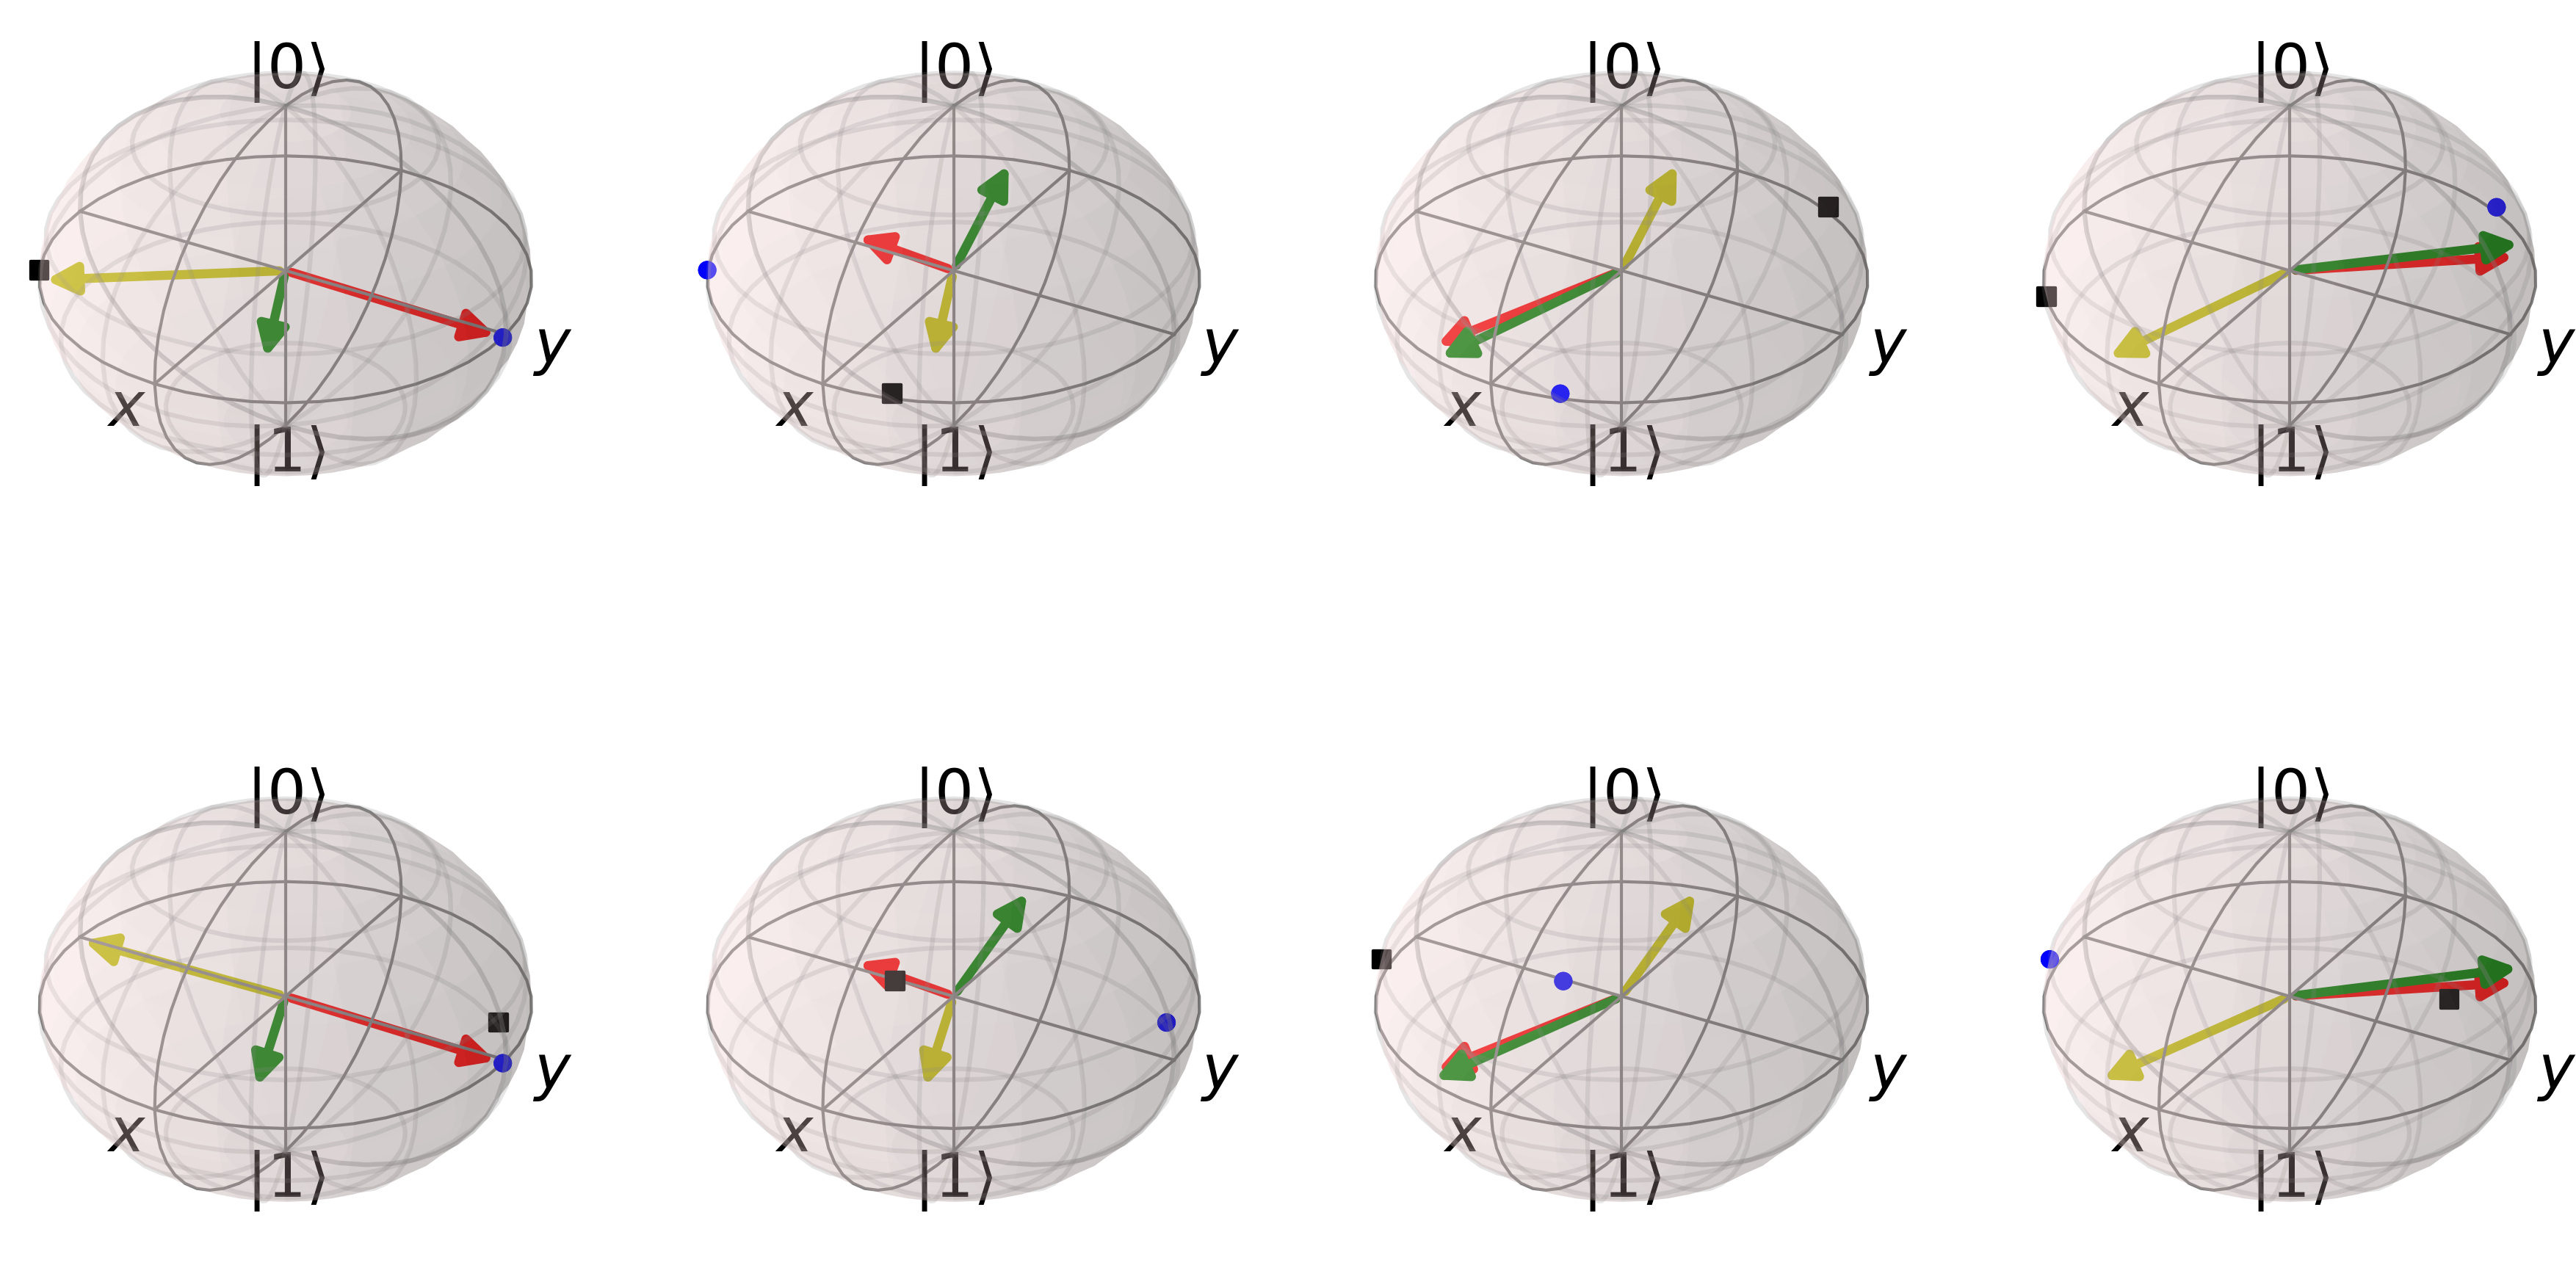
\includegraphics[width=\textwidth]{img/bloch_worst_crop}
		\caption{$W_{opt} = 3.06, W_{pred} = -2.65$}
		\label{bloch_worst}
	\end{subfigure}
	\caption{\textbf{(a)} We plot the evolution of a single sample from the test set for $N=5$ and $\Delta \mathrm{T} = 5$. For this sample we have $W_{opt} = 3.03, W_{pred} = 1.11$. Each Bloch sphere shows $\rho_S^i$ (blue dot), $\rho_S^{i+1}$ (black square), the partial system Hamiltonian acting only between system and Drive $H_{DS}^i$ (red vector) as well as $H_{ST}^i$ (yellow vector) and $H_{ST}^{i+1}$ (green vector). \textbf{Top row:} we plot the system dynamics for the Transducer series generated by the optimiser for $i \in [1, N - 1]$. In the optimal case, $H_{ST}^i$ is chosen such that $\rho_S$ remains near the x-y-plane for all times and $\Tr{\rho_S^{i+1} H_{DS}^i}$ is large. \textbf{Bottom row:} we plot the dynamics for the same Drive protocol with Transducer qubits predicted by the bidirectional LSTM. The overall difference of $\rho_S$ to the x-y-plane is larger. As shown in Figure \ref{bilstmbox}, $\theta_T$ is often set to $\frac{\pi}{2}$ which maximises the strength of $H_{ST}$ as can be seen in all Bloch spheres in the bottom row. In this case, the $H_{DS}$ are chosen by the network to be antiparallel, irrespective of the current system state.
	\textbf{(b)} We show the same plot as in (a) for the worst performing sample from the test set to illustrate a shortcoming of the model. As can be seen from the yellow and green vectors, the predictions for $j \in [2, N]$ are very close to the optimal solutions. However, the first Transducer prediction is wrong, leading to a deviation from the optimal system dynamics.}
	\label{n_5_blochs}
\end{figure}

%\begin{figure}
%	\centering
%	\begin{subfigure}{0.32\textwidth}
%		\centering
%		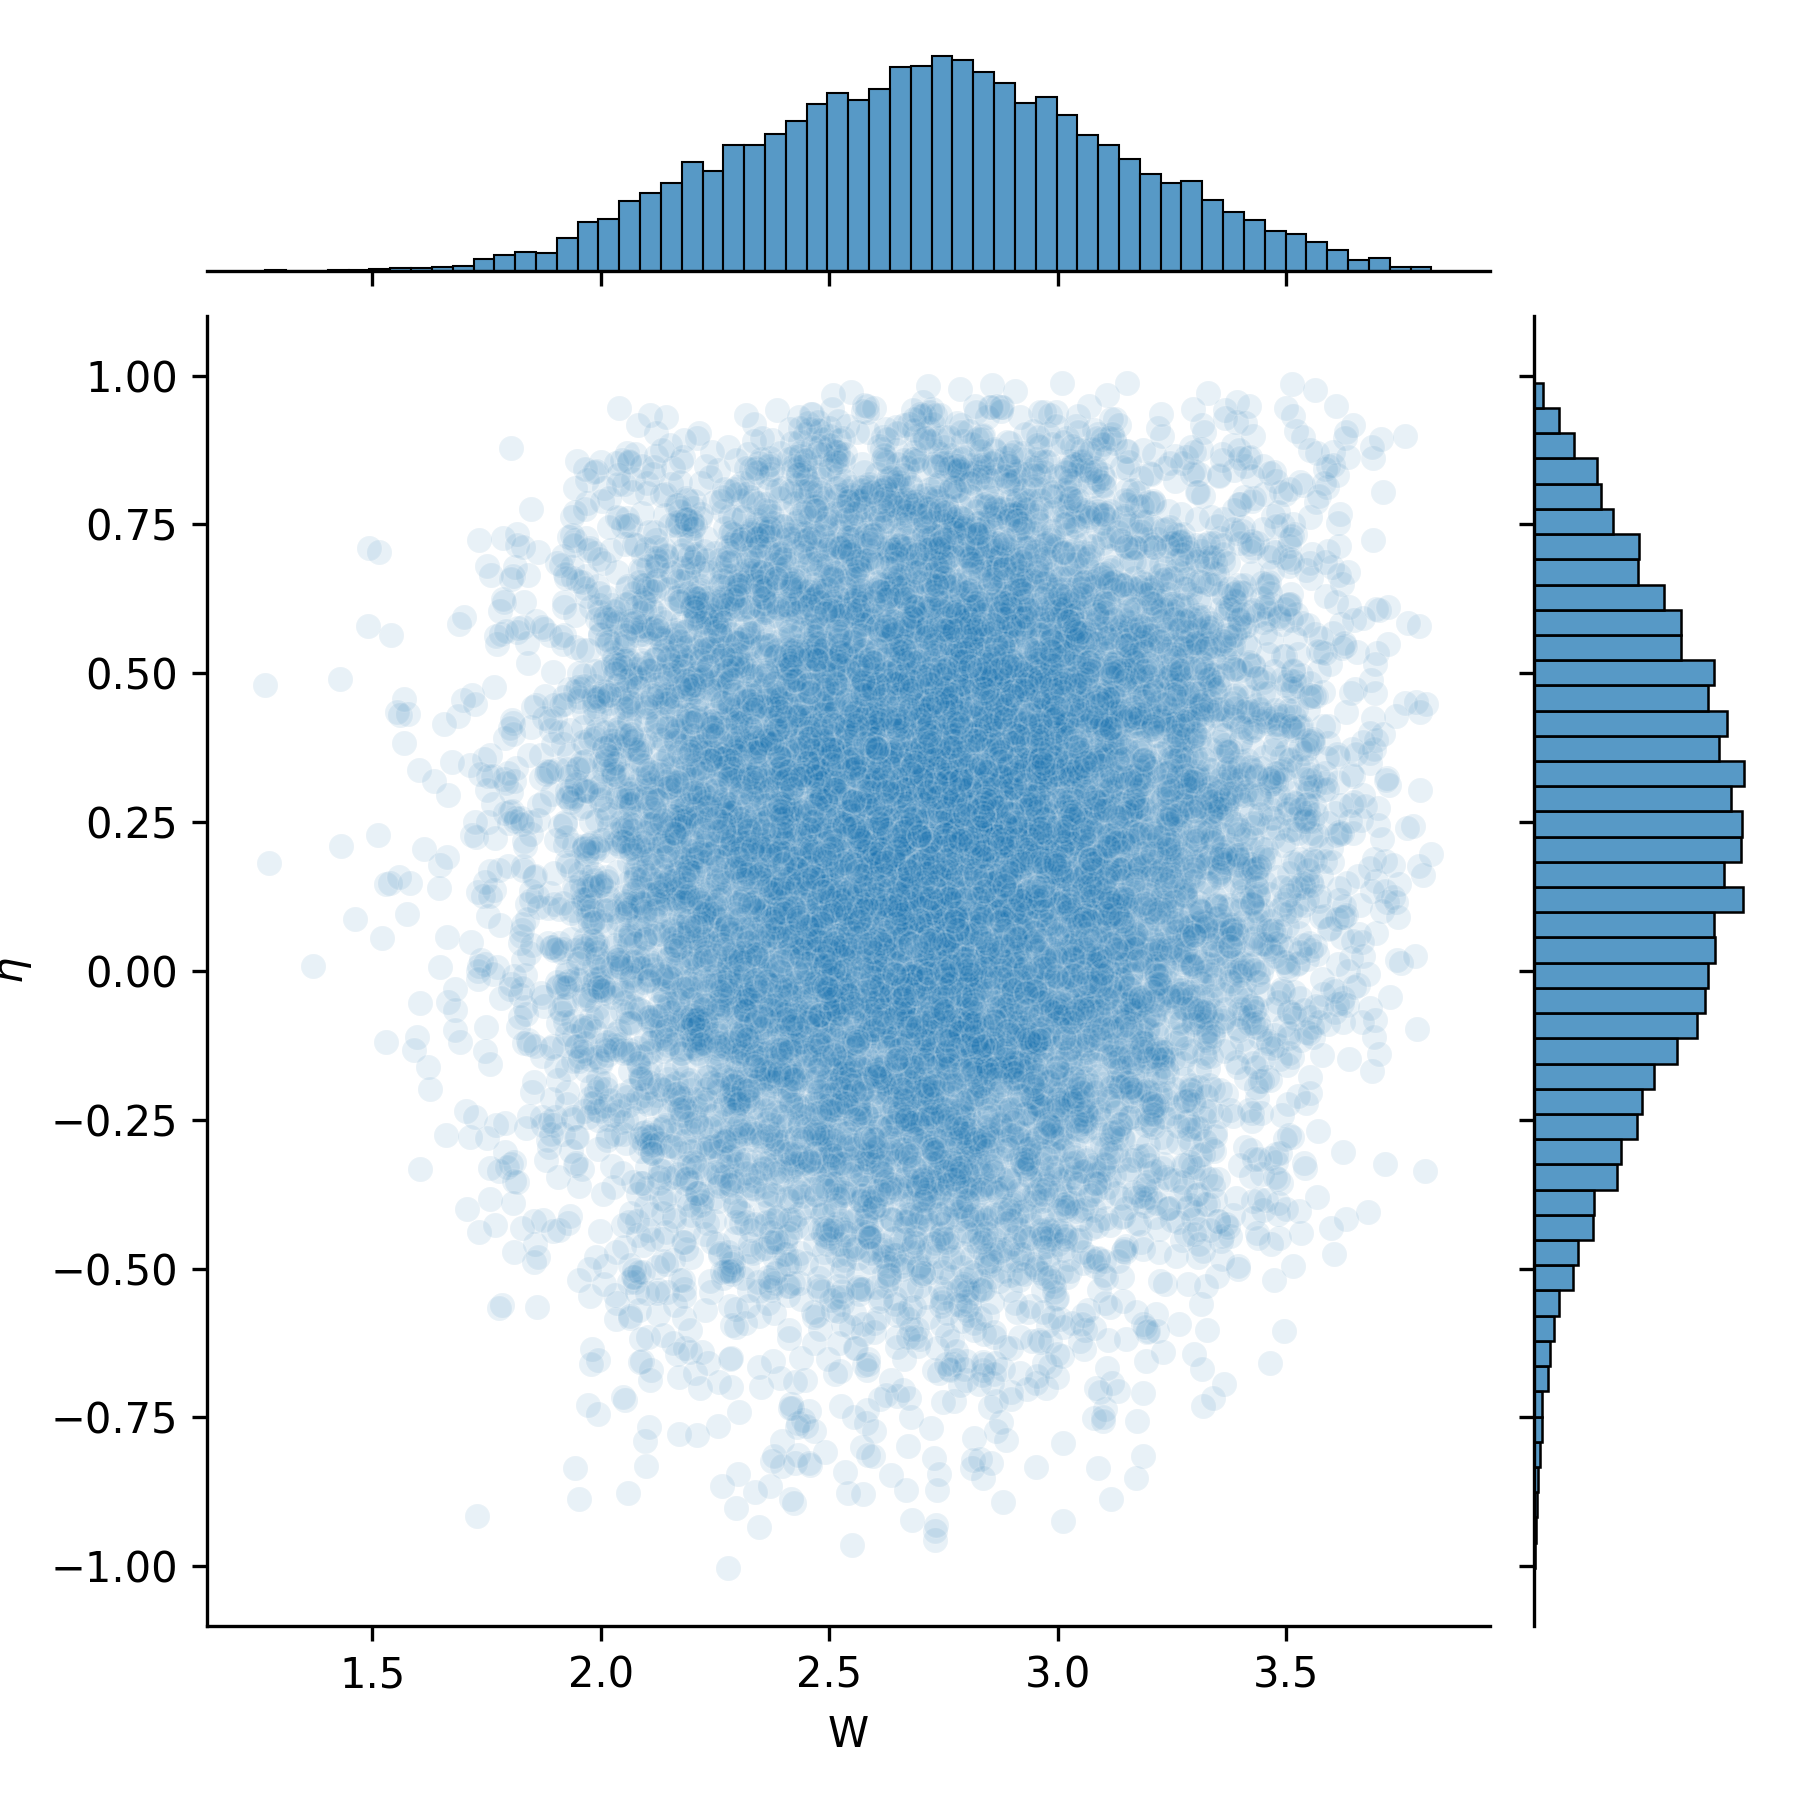
\includegraphics[width=\textwidth]{img/work_dist_n5_eigen_ann}
%		\caption{FCANN}
%		\label{}
%	\end{subfigure}
%	\begin{subfigure}{0.32\textwidth}
%		\centering
%		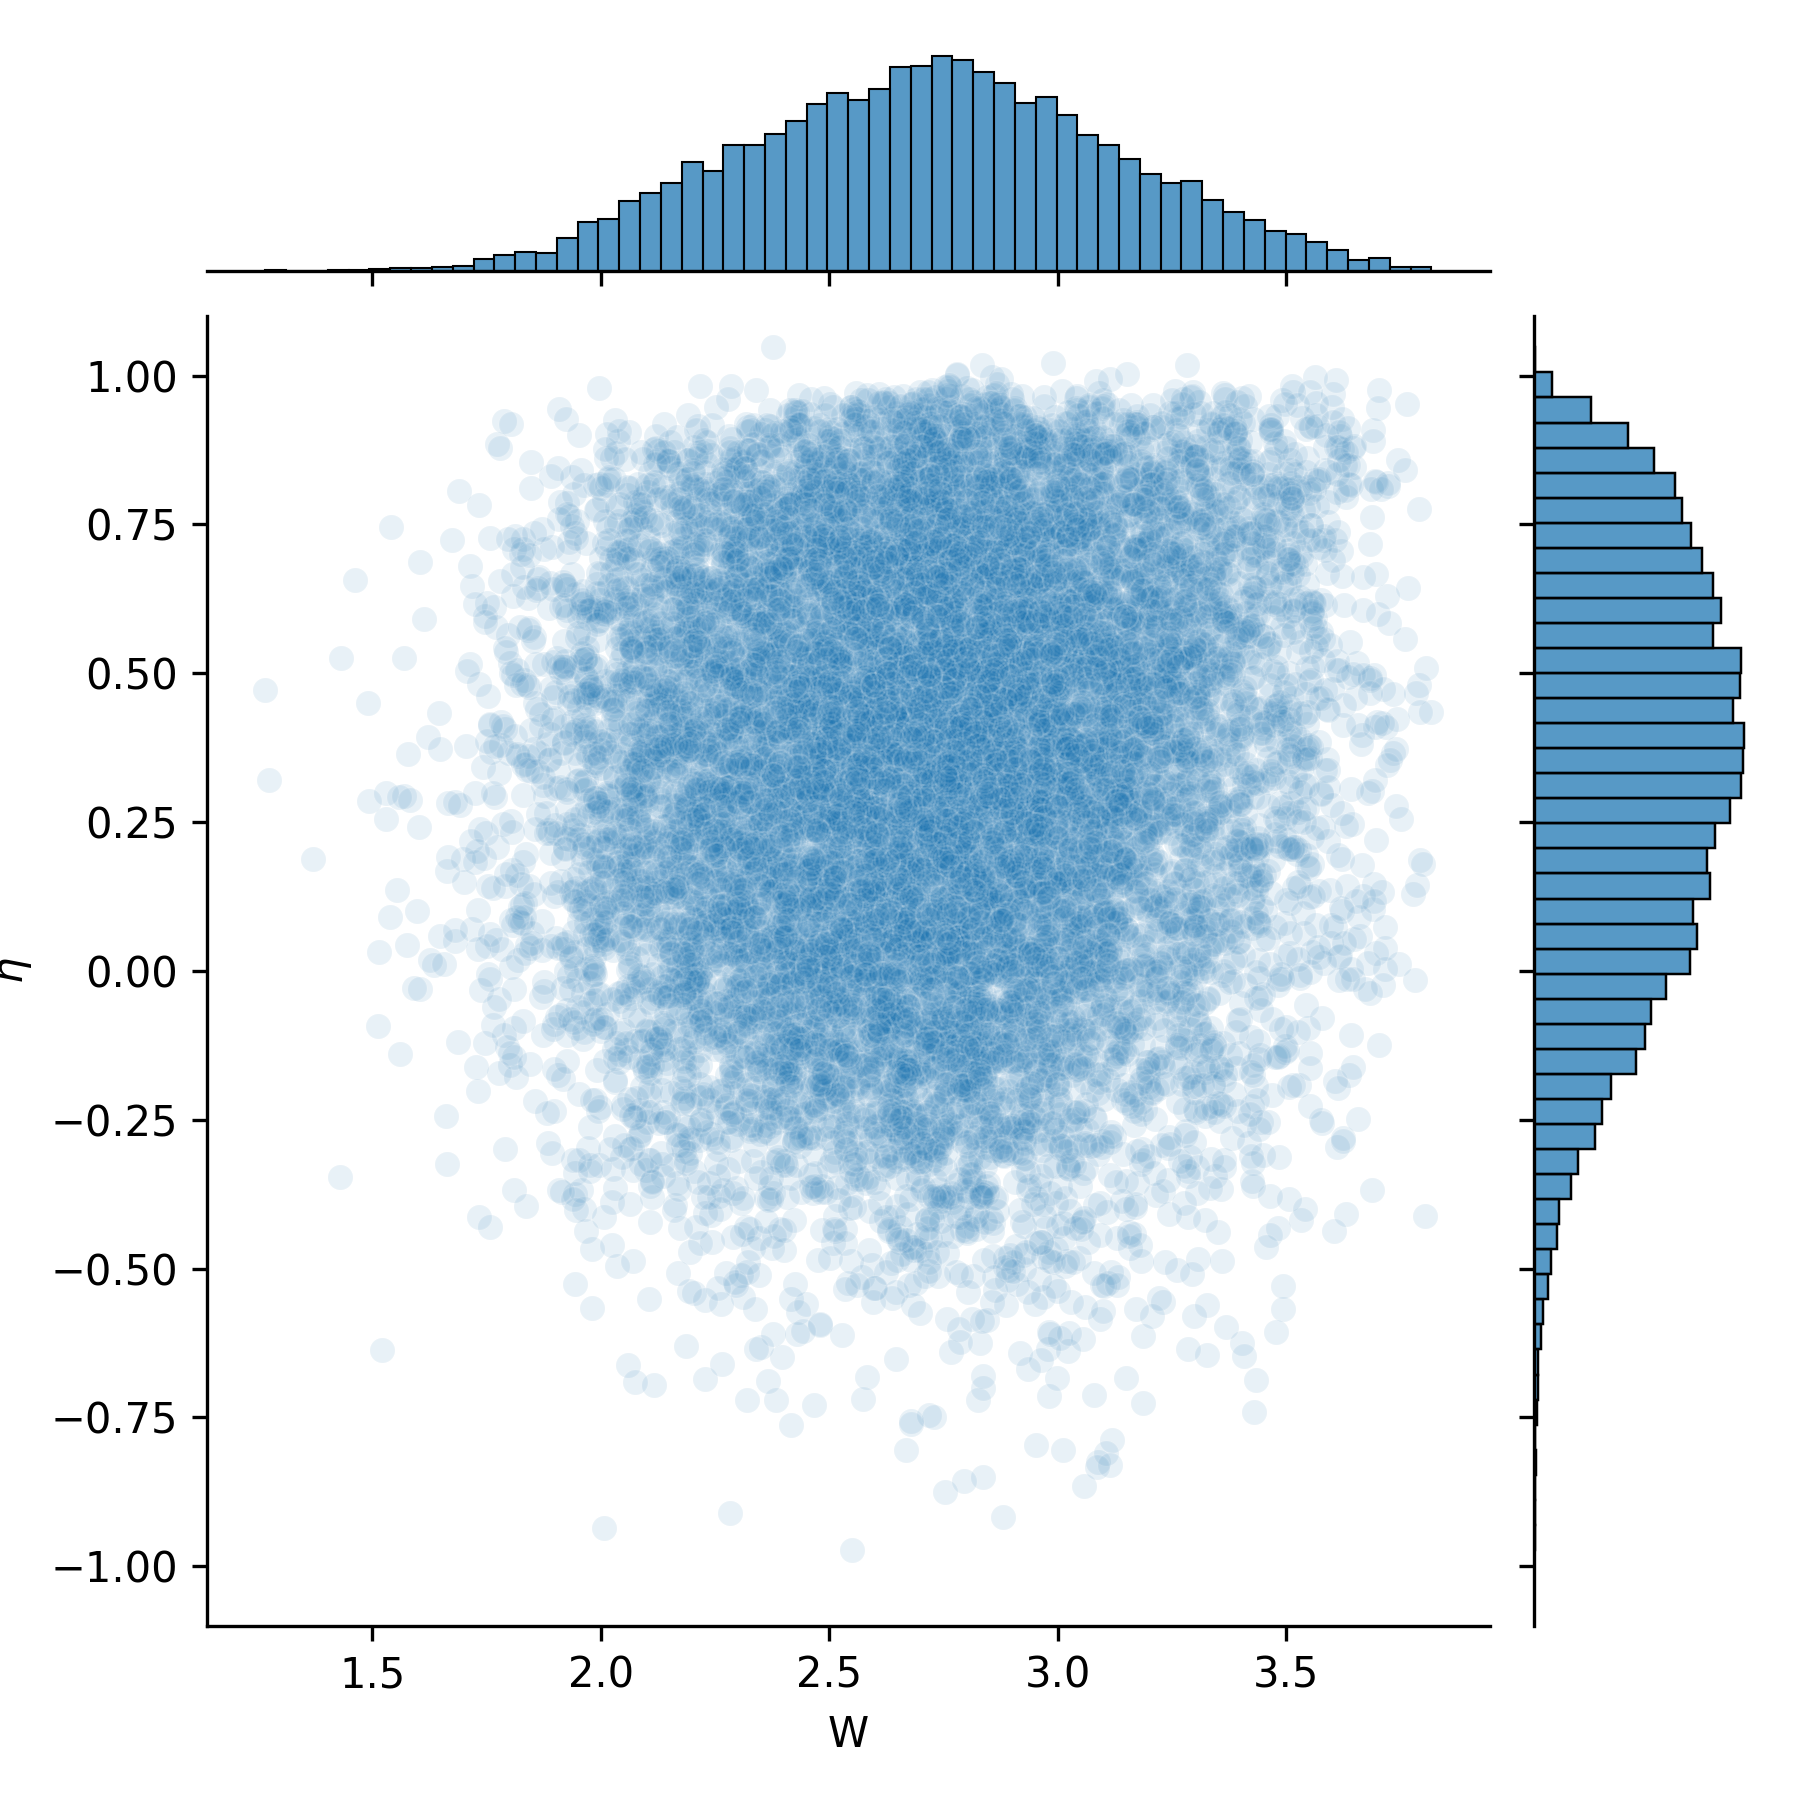
\includegraphics[width=\textwidth]{img/work_dist_n5_eigen_bi}
%		\caption{Bidir. LSTM}
%		\label{}
%	\end{subfigure}
%	\begin{subfigure}{0.32\textwidth}
%	\centering
%	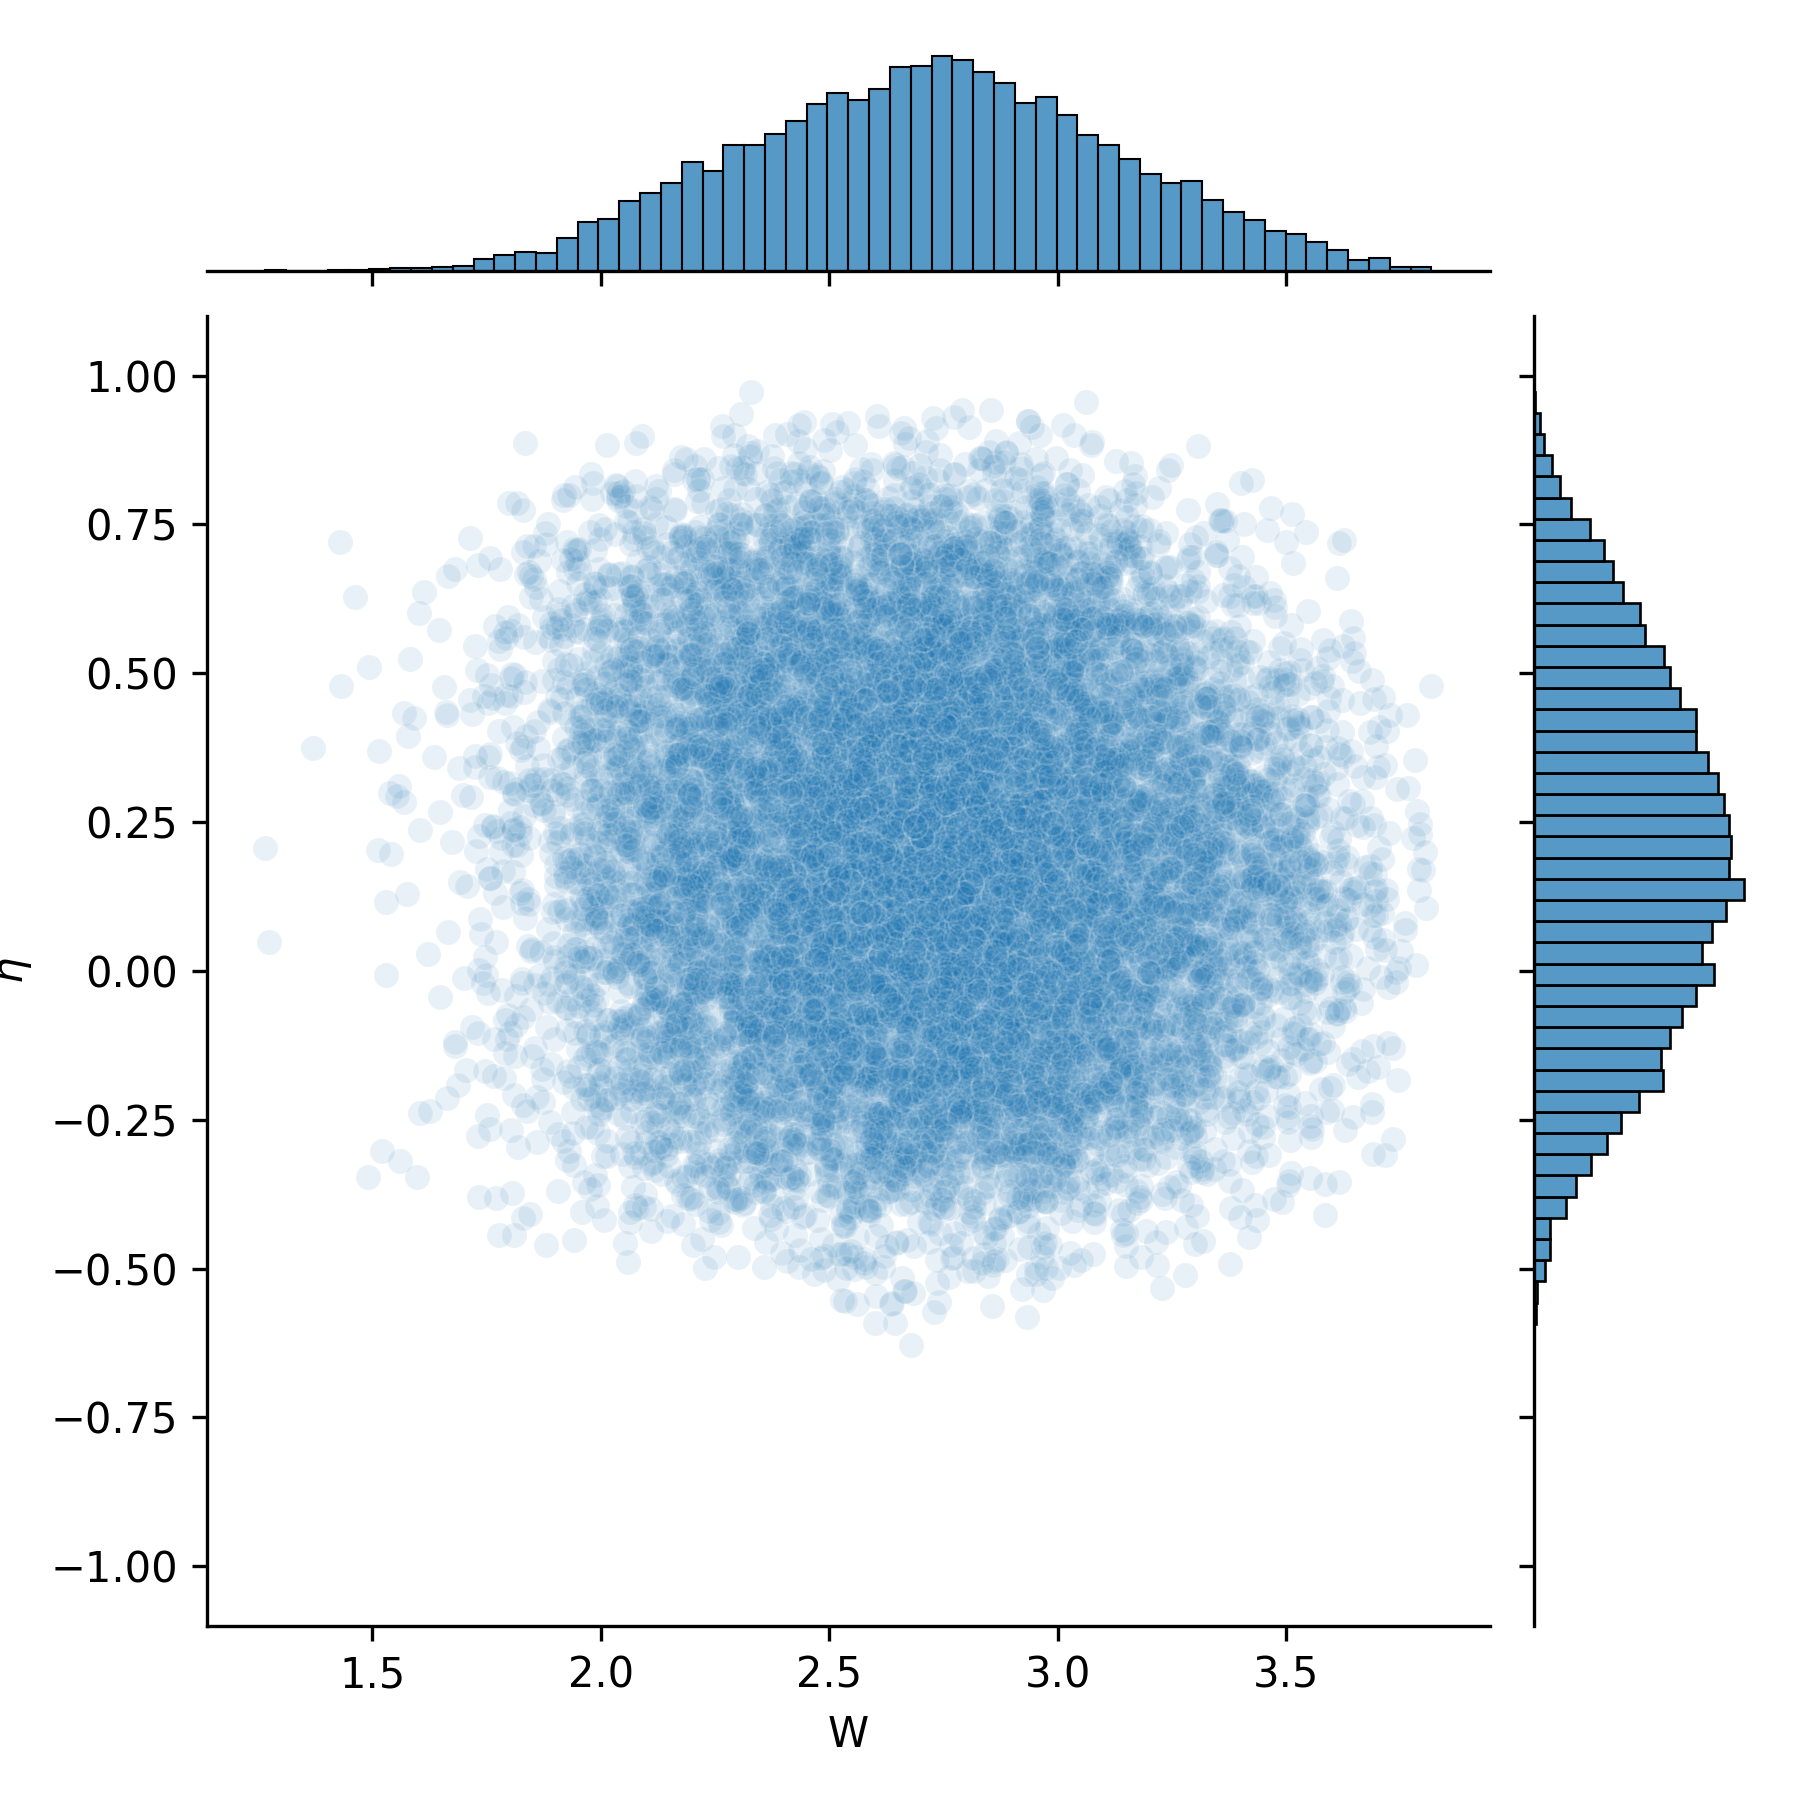
\includegraphics[width=\textwidth]{img/work_dist_n5_eigen_uni}
%	\caption{Unidir. LSTM}
%	\label{}
%\end{subfigure}
%	\caption{We plot the efficiency $\eta$ of each data point in the test set over its optimal work output $W$ for the three network architectures and $\rho_0 = \ket{+}\bra{+}$. The top and right plots on each graph are histograms for $W$ and $\eta$ respectively.}
%	\label{}
%\end{figure}

Figure \ref{bilstmbox} shows the prediction of the bidirectional LSTM and optimal values for the trajecto-ries of each data point in the test set.
There is a notable difference in the predictive quality between the first four qubits and the last one: for the final qubit the dynamics after the work extraction step are inconsequential.
It is therefore beneficial to maximise the strength during the final switching, i.e. setting $\theta_T^N = \frac{\pi}{2}$, to maximise its work output.
Additionally $\phi_T^N$ is should be set so that $H_{ST}^N$ is antiparallel to $\rho_S^N$ on the Bloch sphere.



\begin{figure}
	\centering
	\begin{subfigure}{0.32\textwidth}
		\centering
		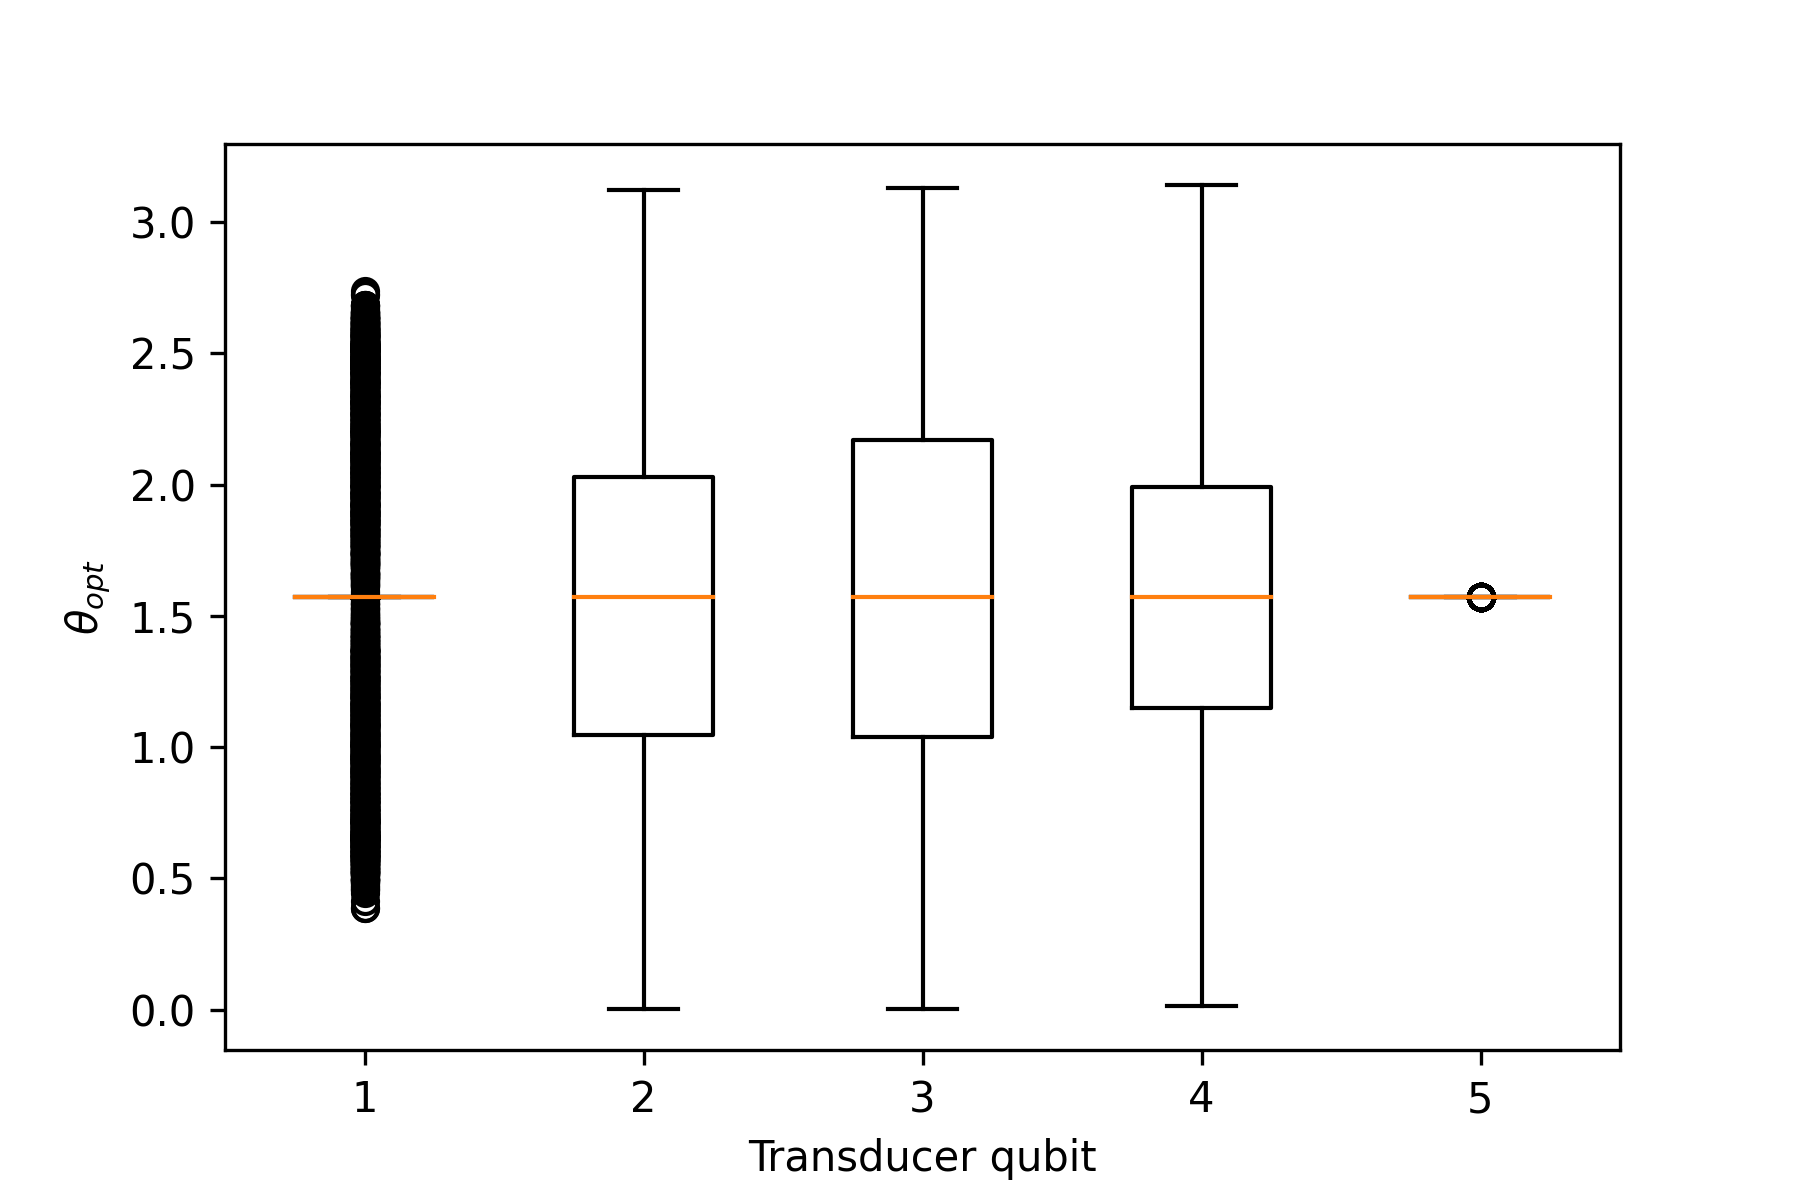
\includegraphics[width=\textwidth]{img/theta_opt_box}
	\end{subfigure}
	\begin{subfigure}{0.32\textwidth}
		\centering
		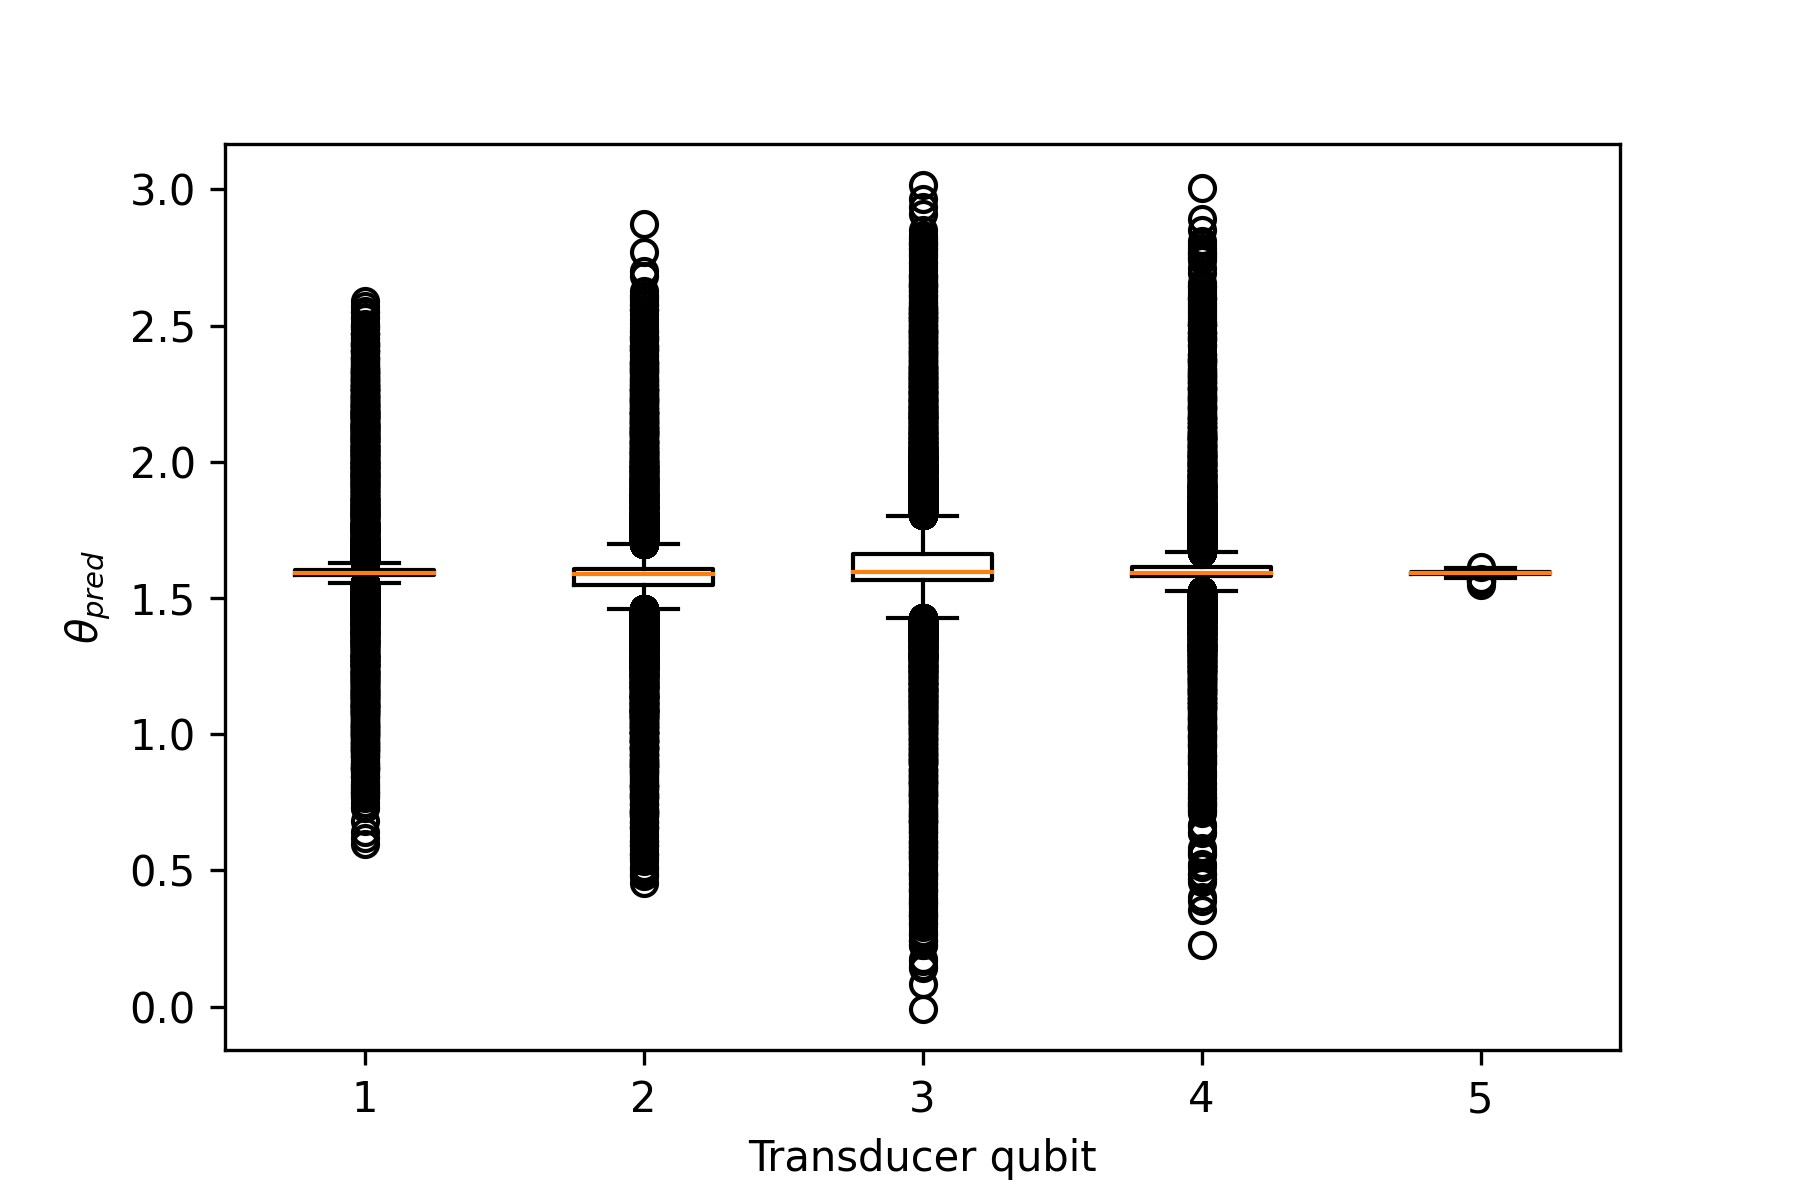
\includegraphics[width=\textwidth]{img/theta_pred_box}
	\end{subfigure}
	\begin{subfigure}{0.32\textwidth}
		\centering
		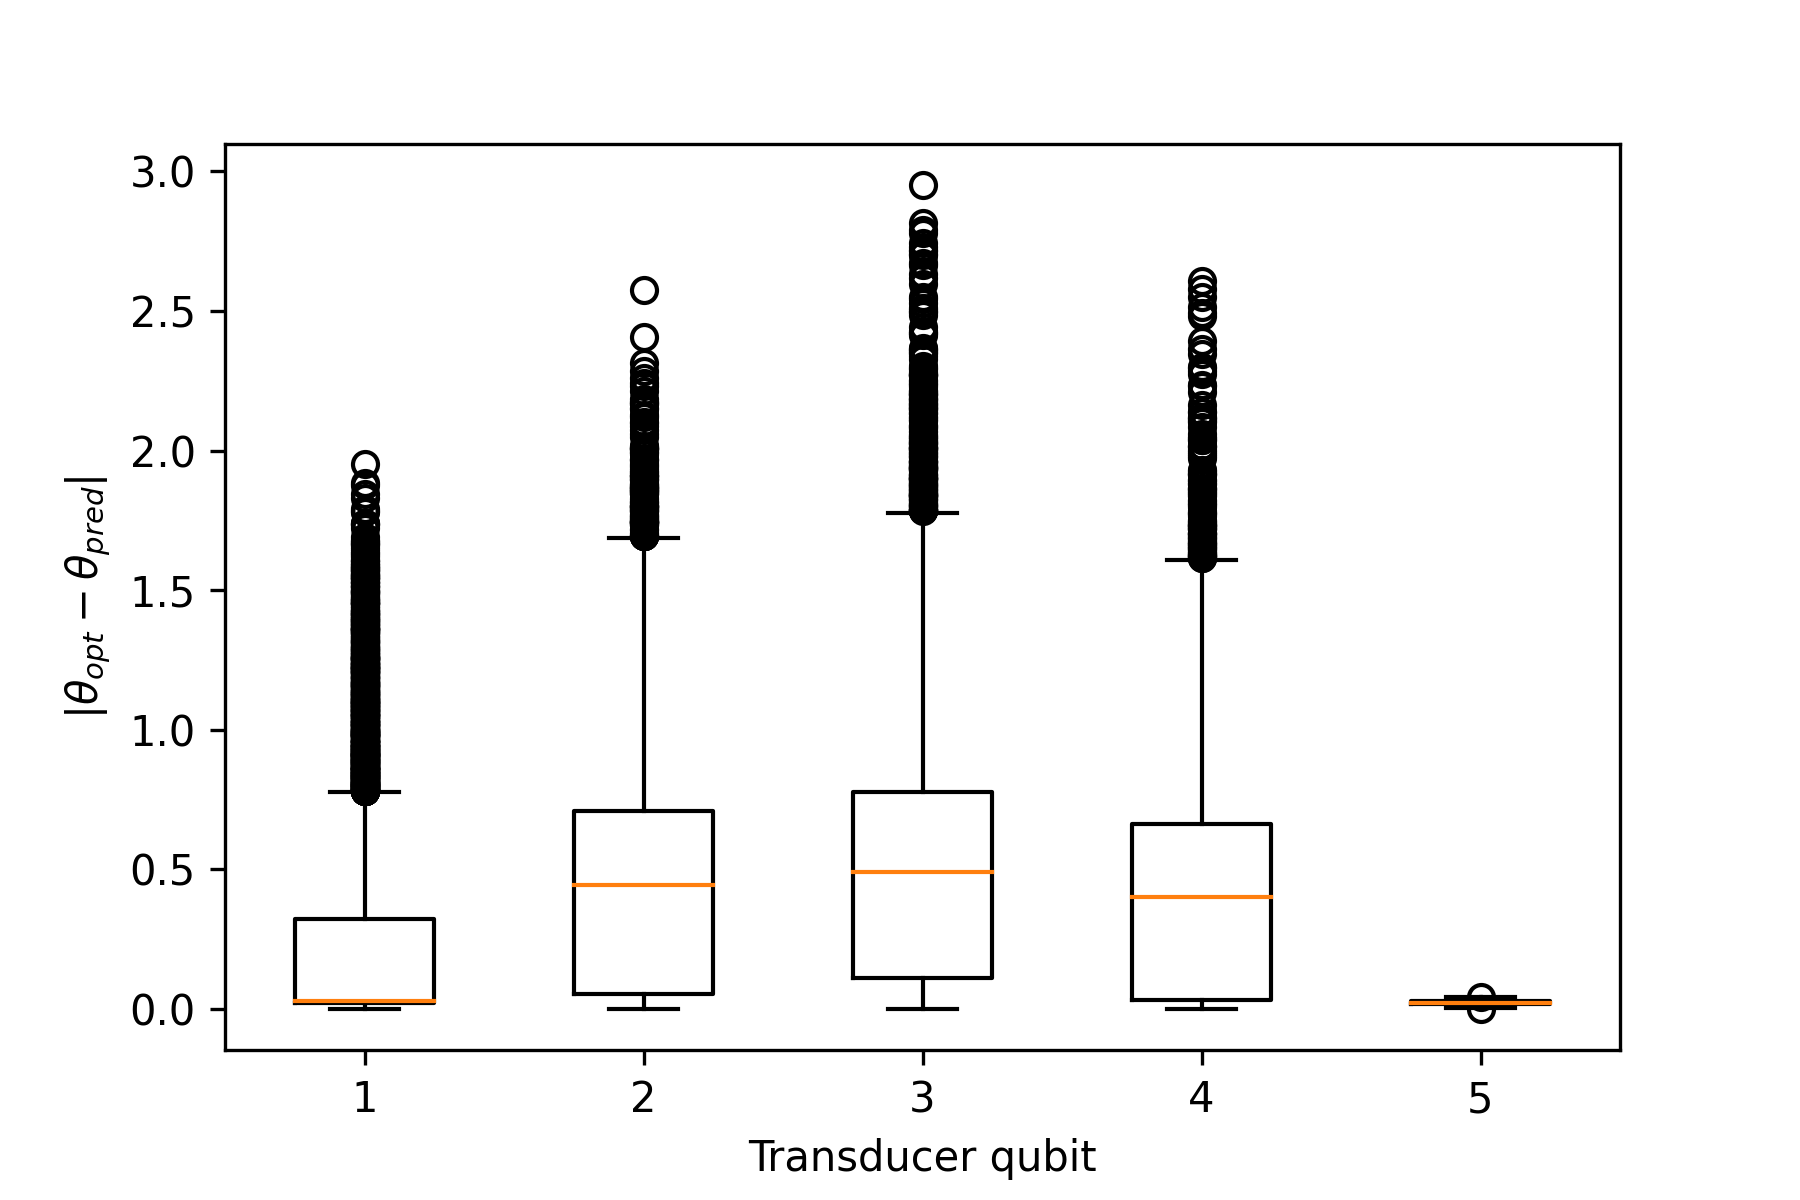
\includegraphics[width=\textwidth]{img/delta_theta_box}
	\end{subfigure}
	\begin{subfigure}{0.32\textwidth}
	\centering
	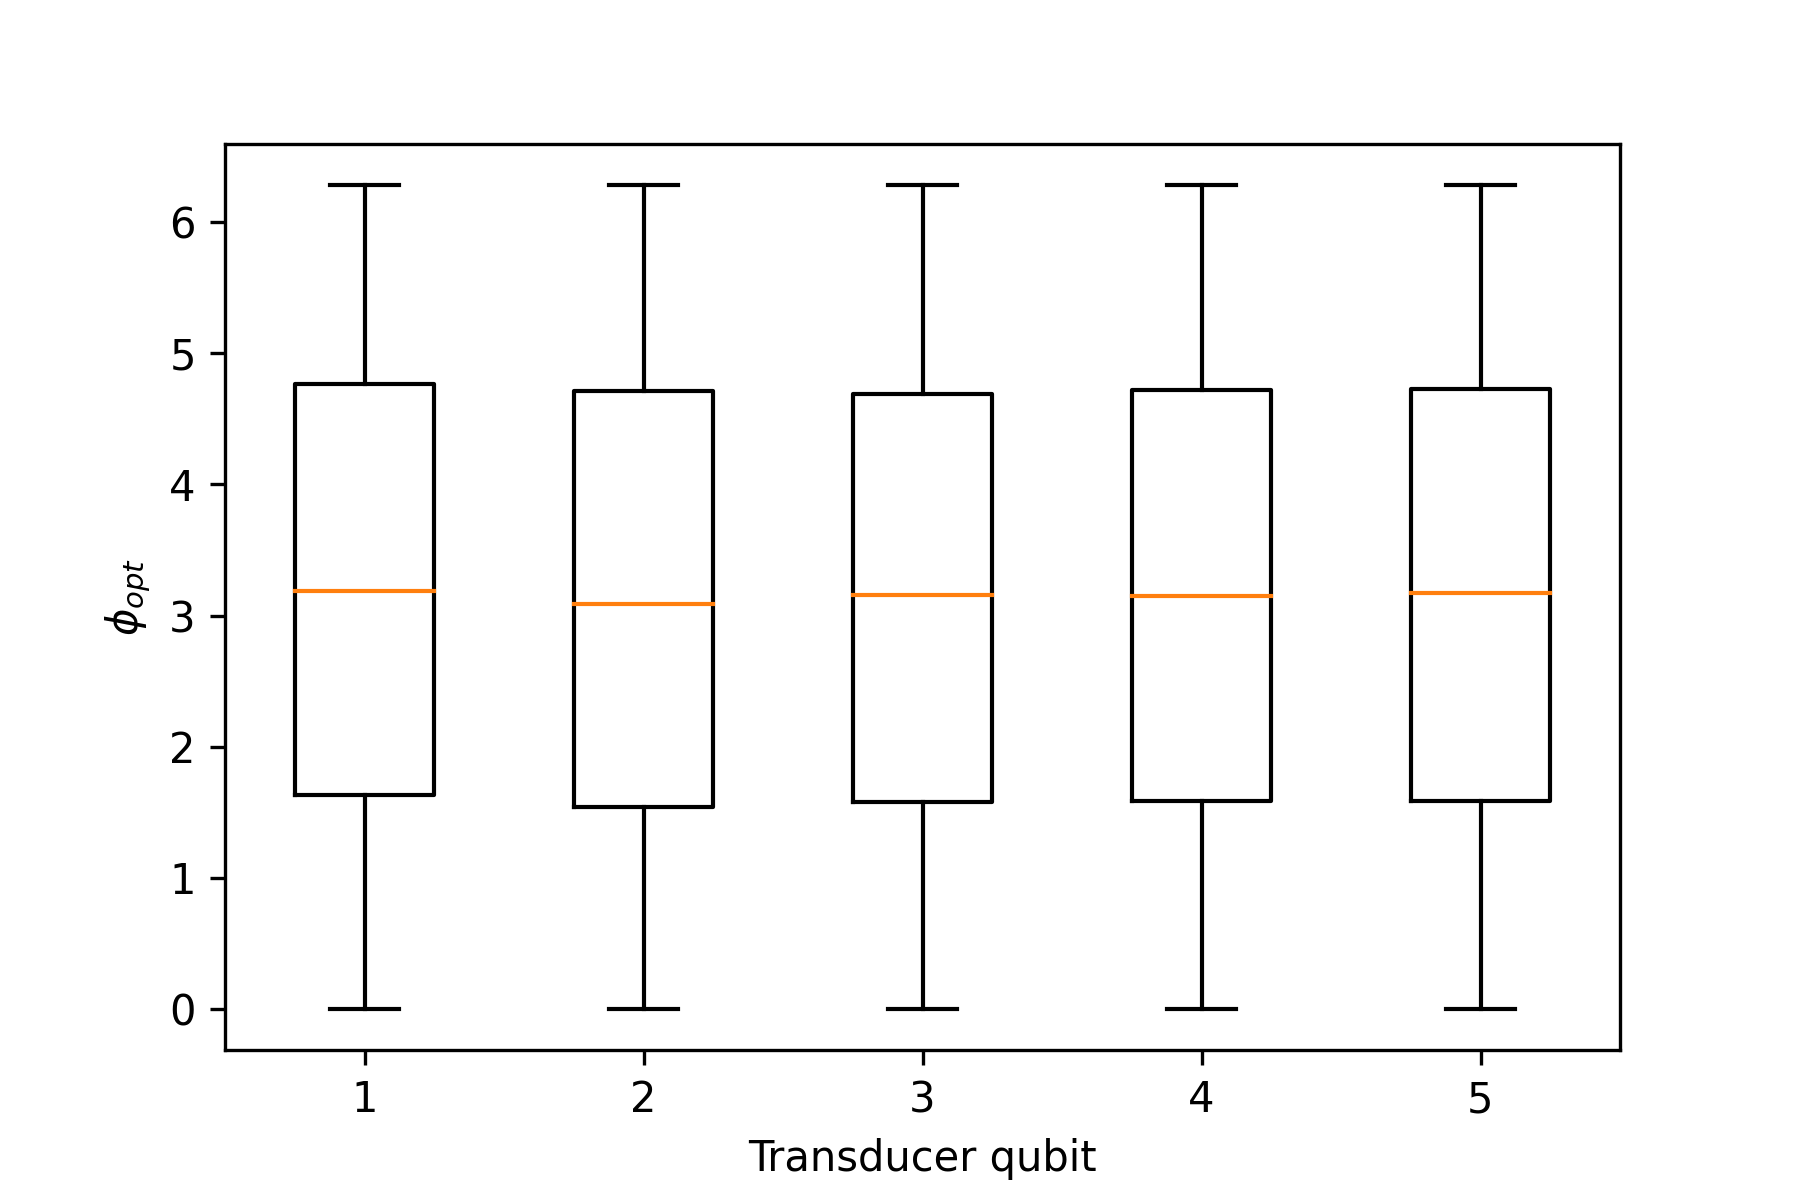
\includegraphics[width=\textwidth]{img/phi_opt_box}
\end{subfigure}
\begin{subfigure}{0.32\textwidth}
	\centering
	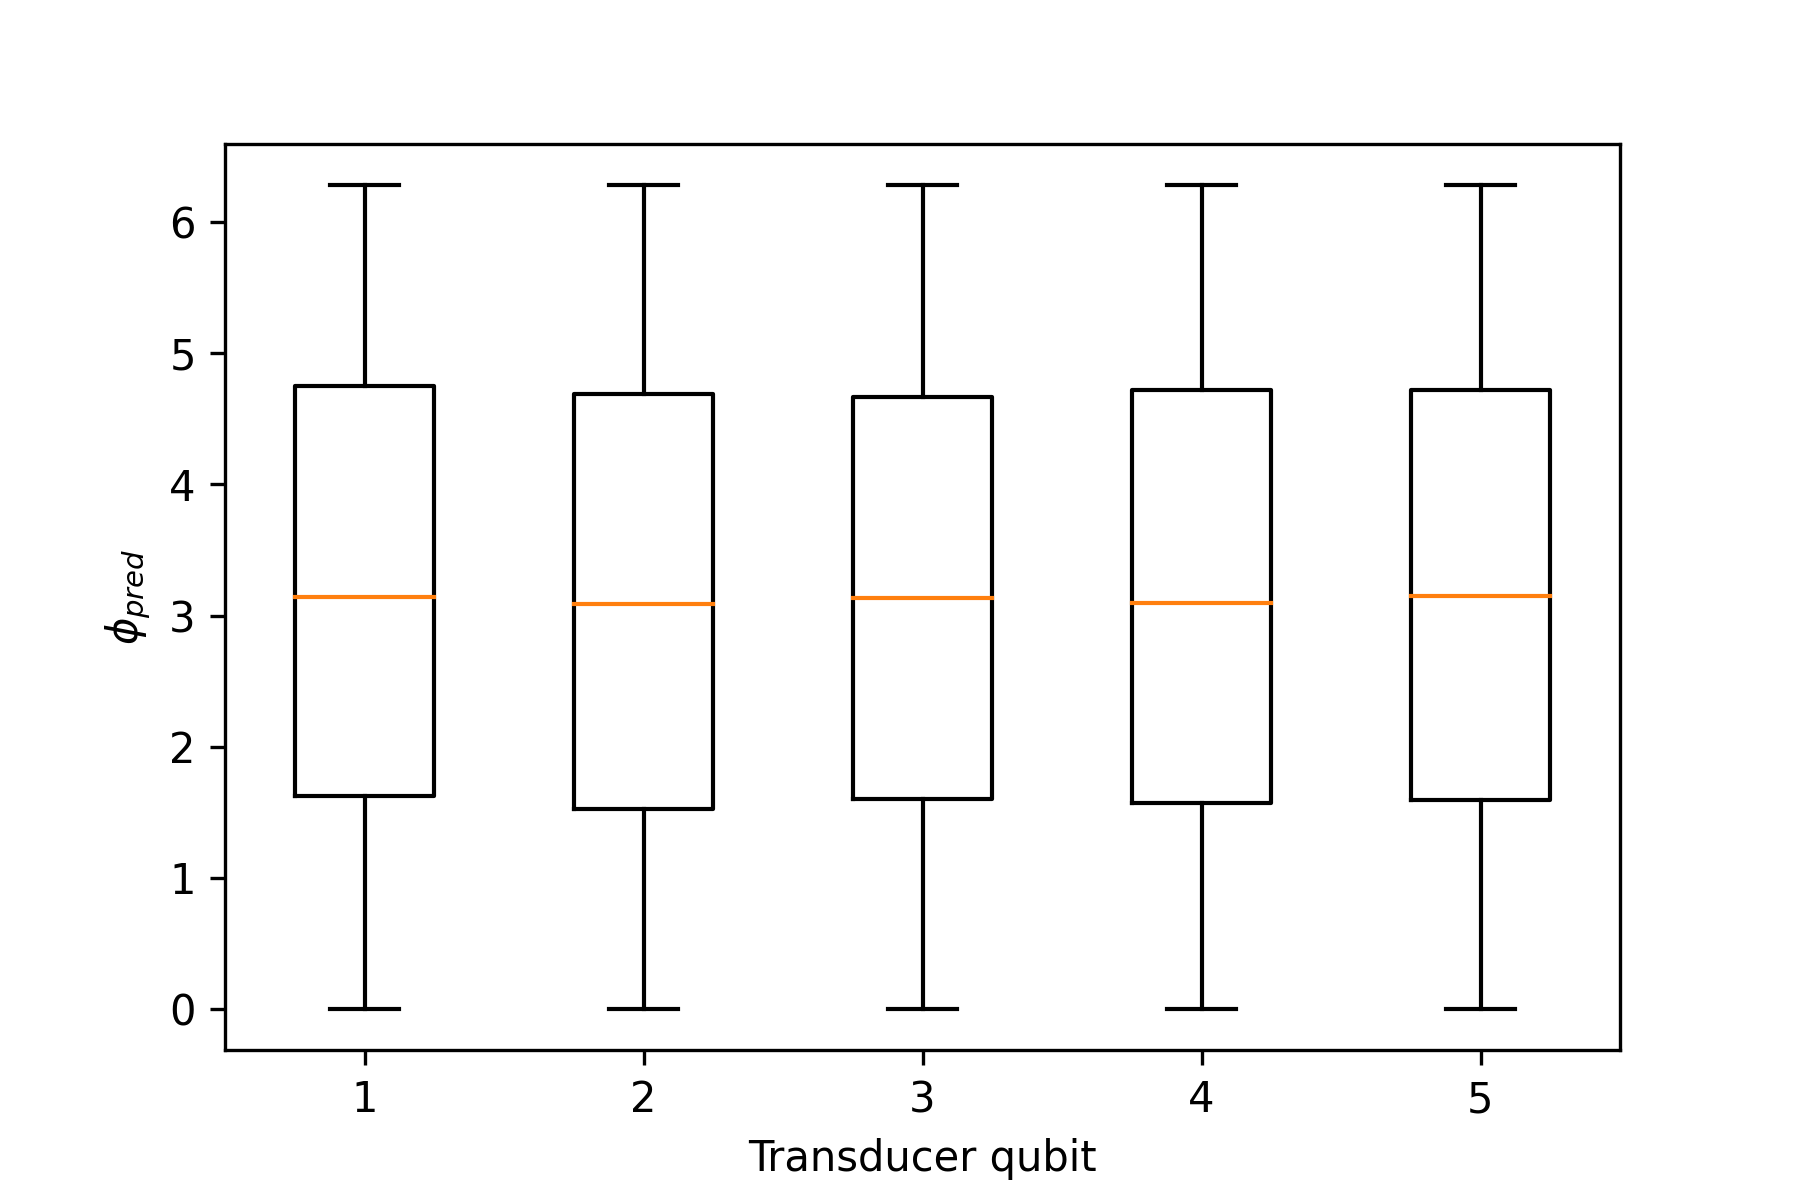
\includegraphics[width=\textwidth]{img/phi_pred_box}
\end{subfigure}
\begin{subfigure}{0.32\textwidth}
	\centering
	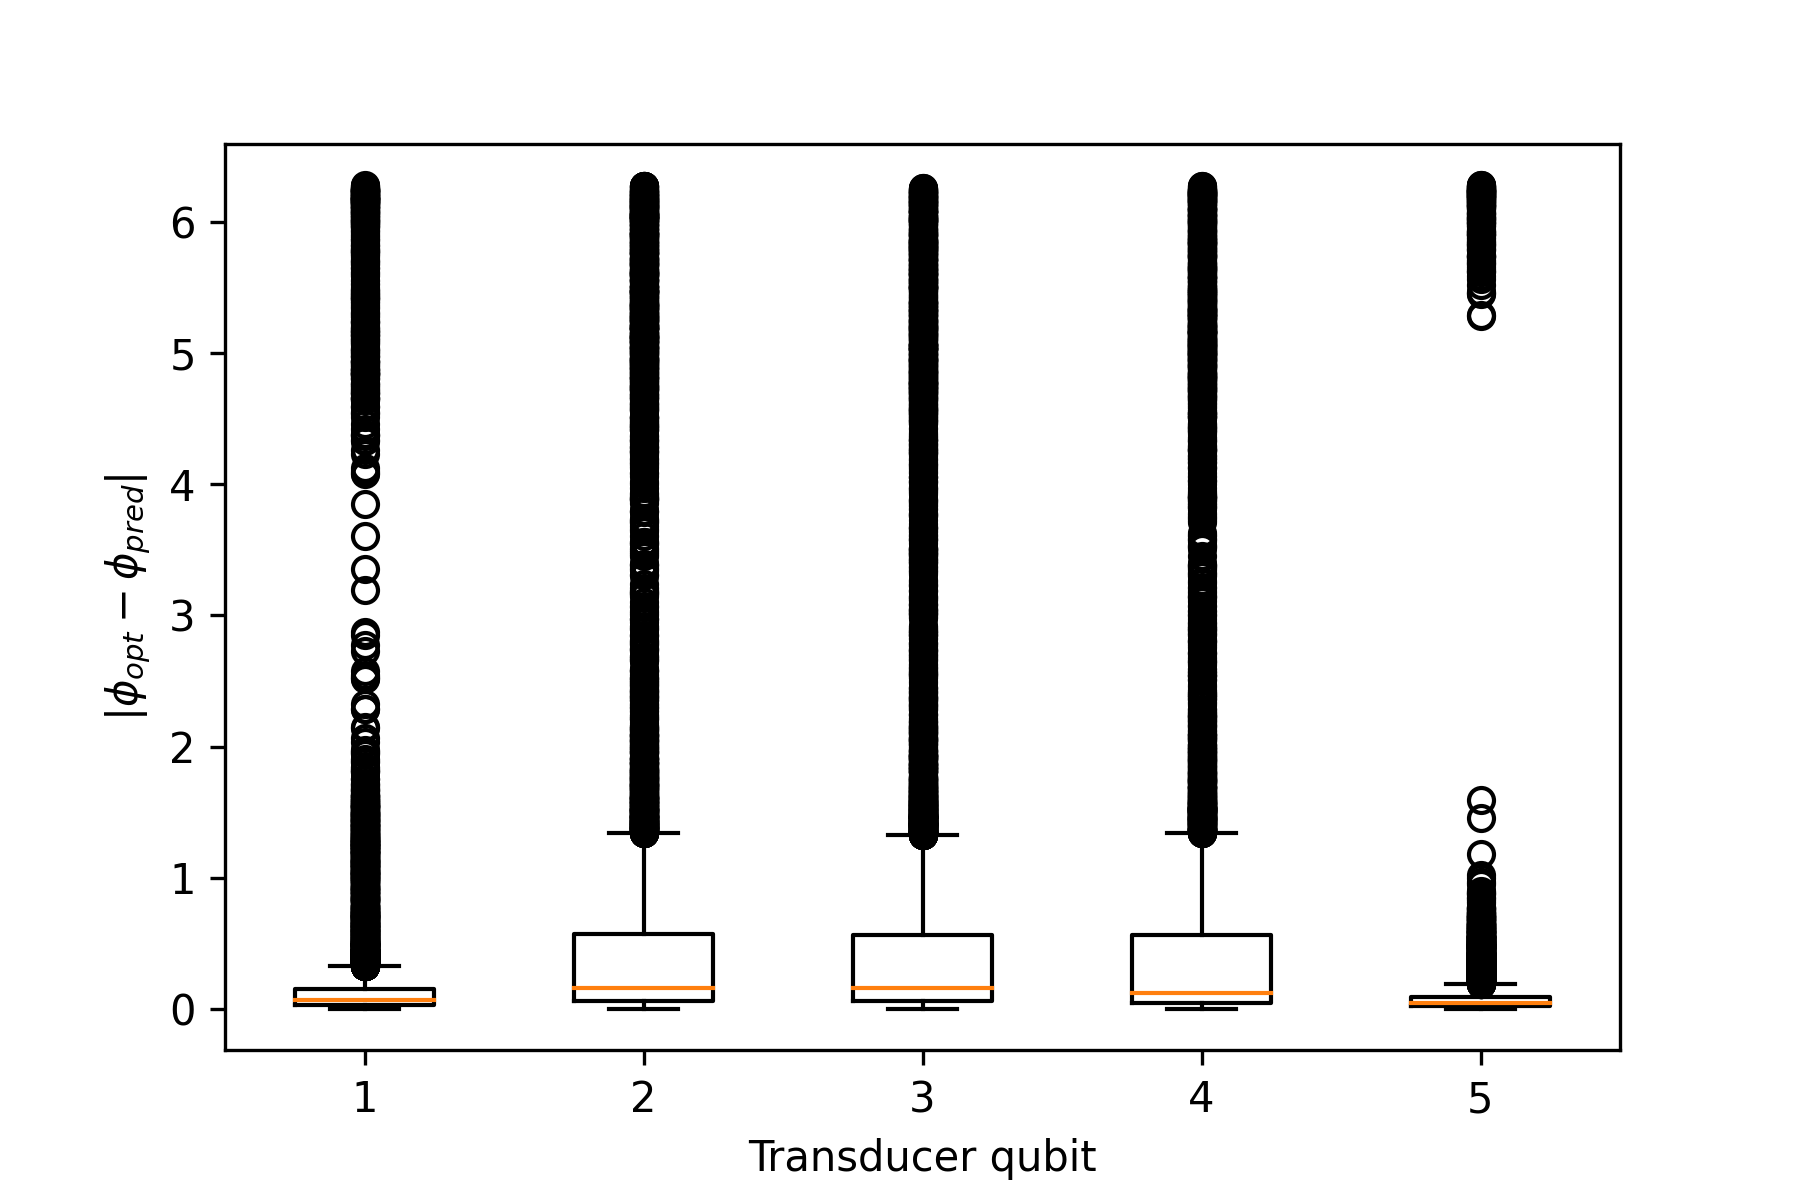
\includegraphics[width=\textwidth]{img/delta_phi_box}
\end{subfigure}
\caption{\textbf{Top row:} for the bidirectional LSTM network and $\Delta \mathrm{T} = 5$, we plot boxplots of the optimal, predicted and absolute differences of $\theta_T$ for the five qubits of each trajectory in the test set. The prediction for $\theta_T^N$ is very good as the optimal solution is to set it to $\frac{\pi}{2}$ in all cases to maximise the work output of the final step. The prediction for $\theta_T^0$ is reasonably good as well, as the optimal solution is again $\frac{\pi}{2}$ in a majority of trajectories. The network is unable to predict the three central qubits, with median absolute differences of approximately $0.5$. \textbf{Bottom row:} we plot the same quantities as above for the Transducer azimuth $\phi_T$.}
\label{bilstmbox}
\end{figure}